\chapter{Methods}
\label{sec:methods}


%%%%%%%%%%%%%%%%%%%%%%%%%%%%%%%%%%%%%%%%%%%%%%%%%%%%%%%%%
\section{Feature extraction and data preparation}
\label{sec:methods:data}

After we extract features from the data described in section~\ref{sec:introduction:data}, it must be labeled, balanced and split.

\subsection{Data labeling}

Supervised machine learning requires labeled data to train the models on. Sounds from the NIGENS database come already labeled, so there is no extra work to do here. However labels must be arranged in a readable and adapted format.

For each sound, the class is stored both as a scalar from $0$ to $11$, as well as an array of size 12 containing only zeros and a one for the active class. The corresponding localization is also stored as scalars (in radians and degrees) and as an array of size 72. Both the scalar and the vector representations were used in the training and testing process of clean sounds.

Mixed sounds were labeled using a technique for exploiting multitask learning and combining both information as shown in figure \ref{fig:methods:label}. Localization vectors are presented horizontally for each row. A void class bin completes the information, stating whether the class is active ($0$) or inactive ($1$) in the mixed sound. The resulting matrix is of size $(13 \times 73)$ (for a total of $949$ parameters).
\begin{figure}[htb]
\[
\newcolumntype{P}[1]{>{\centering\arraybackslash}p{#1}}
\begin{array}{cc|c|c|c|P{2.5cm}P{1cm}P{2.5cm}|c|c|}
& \multicolumn{1}{c}{} & \multicolumn{7}{c}{\text{Localization classes ($72$)}} & \multicolumn{1}{c}{\text{Void}} \\
& \multicolumn{1}{c}{} & \multicolumn{7}{c}{\overbrace{\hphantom{\hspace*{9cm}}}} & \multicolumn{1}{c}{\overbrace{\hphantom{\hspace*{1cm}}}} \\
\cline{3-10}
\parbox[c]{2mm}{\multirow{7}{*}{\rotatebox[origin=c]{90}{Identification classes ($13$)}}} & \multirow{7}{*}{\rotatebox[origin=c]{90}{$\overbrace{\hspace*{4cm}}$}} & 0 & 0 & 1 & & \ldots & & 1 & 0 \\
\cline{3-6}\cdashline{7-7}\cline{8-10}
& & 0 & 0 & 0 & & \ldots & & 0 & 1 \\
\cline{3-6}\cdashline{7-7}\cline{8-10}
& & 0 & 1 & 0 & & \ldots & & 0 & 0 \\
\cline{3-10}
& & & & & \multicolumn{1}{l}{\ddots} & \multicolumn{4}{c}{} \\
& & \multicolumn{1}{c:}{\vdots} & \multicolumn{1}{:c:}{\vdots} & \multicolumn{1}{:c|}{\vdots} & \multicolumn{5}{c}{} \\
& & & & & \multicolumn{5}{c}{} \\
\cline{3-5}
& & 0 & 0 & 0 & \multicolumn{5}{c}{} \\
\cline{3-5} \\
\end{array}
\]
\caption{Labeling methods for mixed sounds combining localization and identification}
\label{fig:methods:label}
\end{figure}

\subsection{Feature description}

The features to feed into the machine learning algorithm are ratemaps, amplitude modulation spectrogram based features and interaural level differences. They all are computed using the Two!Ears auditory front-end \parencite{schymuratwo} and all have two channels for each ear signal, except for interaural level differences which only has one channel that sums up both signals information. We changed the feature computation parameters when switching from clean sounds to mixed sounds in order to speed up computation in the system and reuse the features for other purposes. This explains why the obtained features may not have the same size for clean and mixed sounds.

\textbf{Ratemaps}. Log-scaled spectrograms are extracted from all recordings (truncated in windows of 0.5~s) with Hann-window step size of 32~ms along 63 frequency channels between 80~Hz and 8~kHz for clean sounds, and with Hann-windows step size of 21~ms along 50 frequency channels for mixed sounds. Ratemaps can thus be stored as an array of size ($16 \times 63$) for clean sounds and size ($24 \times 50$) for mixed sounds. In the context of bio-inspired methods, ratemaps accurately picture the neural activity in that they represent a map of auditory nerve firing rates \parencite{schymuratwo}.

\textbf{Amplitude modulation spectrograms based features} (AMS). AMS contain several channels for each ear with information of both center frequencies and modulation frequencies for each time frame, which mimics the auditory cortex of mammals \parencite{langner1992periodicity}. The detection of envelope fluctuations is indeed a central aptitude of the human auditory system \parencite{moritz2011amplitude}. They are obtained after both a short-term frequency analysis and a modulation spectrogram \parencite{schymuratwo}. AMS can be stored as arrays of size ($18 \times 16 \times 63$) for clean sounds and of size ($16 \times 16 \times 16$) for mixed sounds.

\textbf{Interaural level differences} (ILD). ILD are a standard feature in machine hearing. It relies on the fact that a sound emitted on the right side of the head will have a higher level at the right ear than at the left ear. ILD are estimated for each individual frequency channel by comparing the frame-based energy of the left and right-ear envelope \parencite{schymuratwo}. ILD can be stored as arrays of size ($32 \times 50$) for mixed sounds. ILD were not computed for clean sounds.

\begin{figure}[htb]
\begin{subfigure}[t]{0.3\textwidth}
	\hspace*{-2cm}
	\centering
	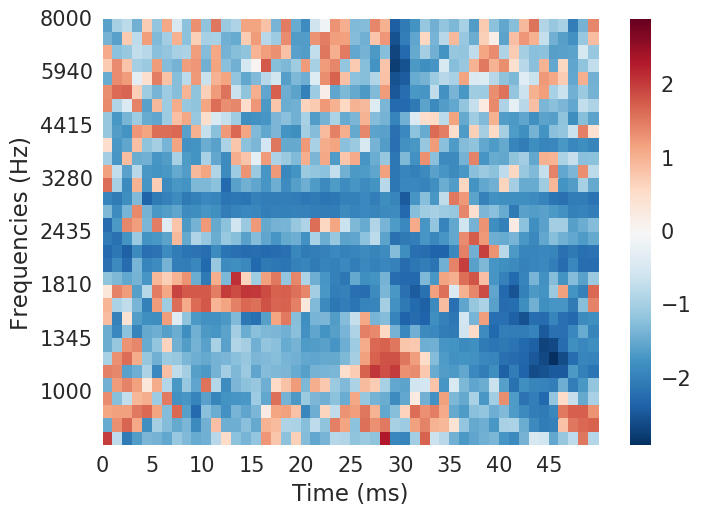
\includegraphics[scale=0.3,valign=t]{images-data/ild}
	\caption{ILD feature}
	\label{fig:methods:ild}
\end{subfigure}~
\begin{subfigure}[t]{0.3\textwidth}
	\hspace*{-0.5cm}
	\centering
	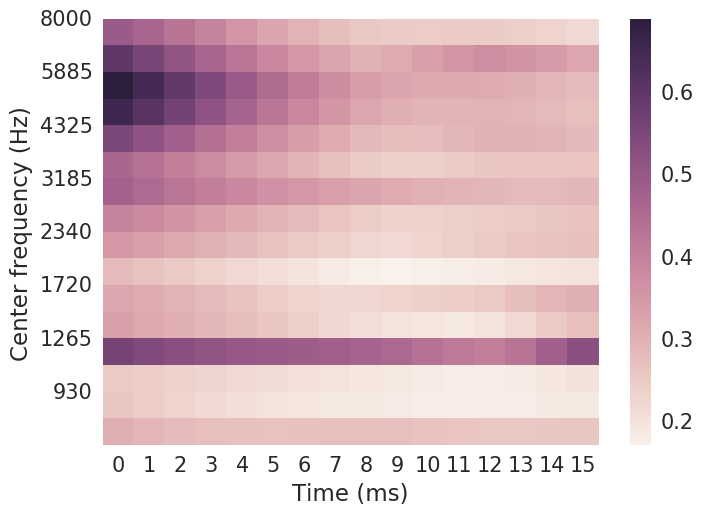
\includegraphics[scale=0.3,valign=t]{images-data/ams}
	\caption{Left-channel first AMS}
	\label{fig:methods:ams}
\end{subfigure}~
\begin{subfigure}[t]{0.3\textwidth}
	\centering
	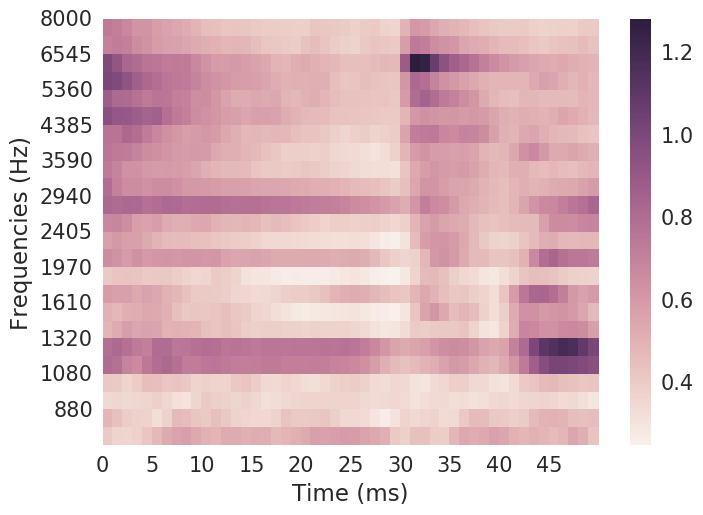
\includegraphics[scale=0.3,valign=t]{images-data/rmp}
	\caption{Left-channel ratemap}
	\label{fig:methods:rmp}
\end{subfigure}
\caption{Features representation for a "phone" recording (ILD, AMS and ratemap)}
\end{figure}

\subsection{Balancing}
\label{sec:methods:balancing}

All types of classes are originally strongly imbalanced for both types of sounds. That means some classes are outnumbered by other classes. That could possibly lead to a bias towards the majority classes, treating minority classes as outliers or even not considering rare events at all. This phenomenon applies to identifications classes (class count in figure~\ref{fig:methods:class_count_clean}), localization classes (azimuths count in figure~\ref{fig:methods:class_count_azimuths}) and number of sources (counted for one specific class in figure~\ref{fig:methods:class_count_sources}).

Balancing is performed by counting each class and fixing a target as the exact class count we want to reach for each class after balancing. Minority classes are artificially oversampled by repeating elements from the class; majority classes are subsampled.
\begin{figure}[htb]
\begin{subfigure}[t]{0.5\textwidth}
	\centering
	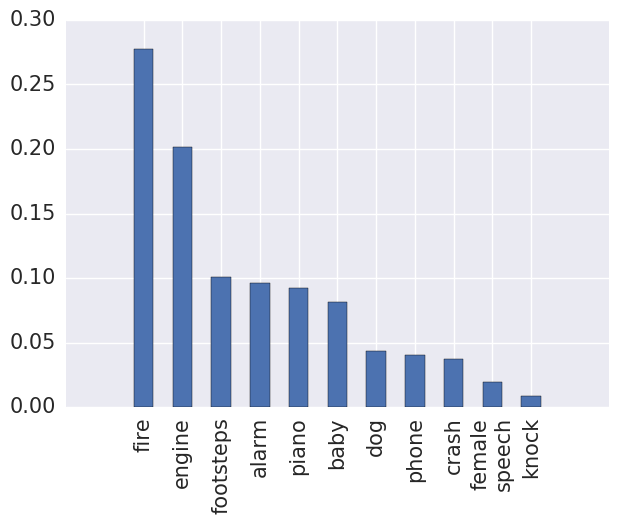
\includegraphics[scale=0.4,valign=t]{images-data/class_count_clean}
	\caption{Identification classes for clean sounds}
	\label{fig:methods:class_count_clean}
\end{subfigure}%
\begin{subfigure}[t]{0.5\textwidth}
	\centering
	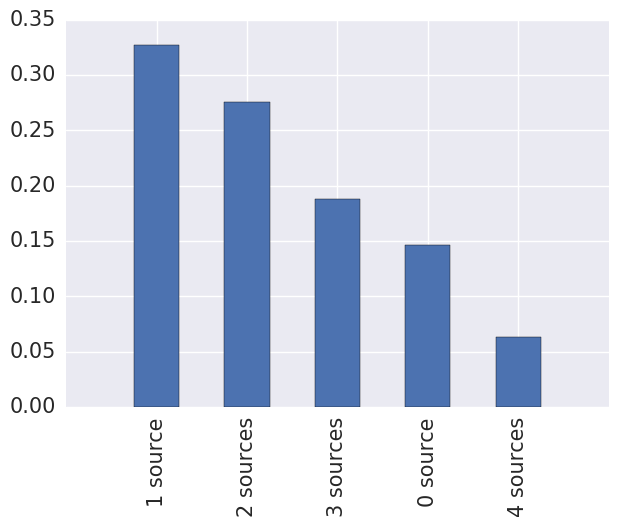
\includegraphics[scale=0.4,valign=t]{images-data/class_count_sources}
	\caption{Co-occurent sources for mixed sounds}
	\label{fig:methods:class_count_sources}
\end{subfigure}
\begin{subfigure}[t]{\textwidth}
	\centering
	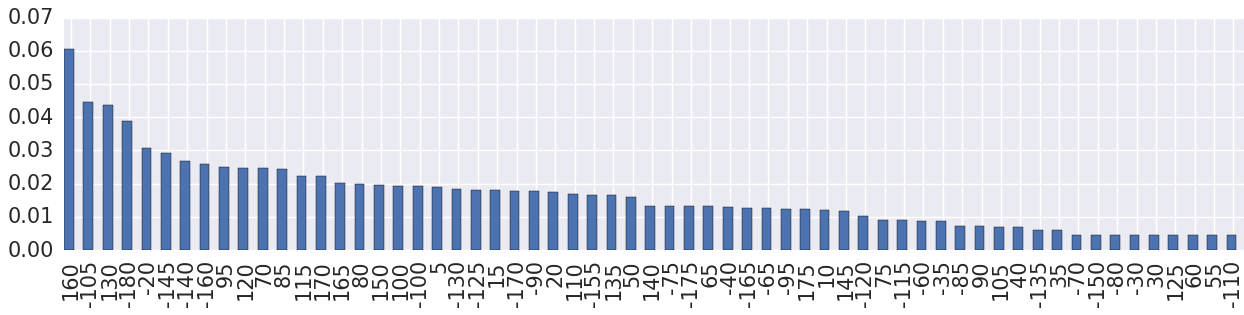
\includegraphics[scale=0.45]{images-data/class_count_azimuths}
	\caption{Distribution of azimuths for the class "alarm" of the mixed sounds (sorted according to frequencies of localization classes)}
	\label{fig:methods:class_count_azimuths}
\end{subfigure}
\label{fig:methods:balancing}
\caption{Percentage ratio of several classes for clean and mixed sounds (while some classes stand out, others are outnumbered)}
\end{figure}

Although balancing was performed for identification classes, it has not been solved on mixed sounds in the azimuth plane. Balancing one class type (\textit{e.g.} azimuths) would indeed tend to imbalance another one (\textit{e.g.} number of sources). That is why azimuth imbalance was not tackled for mixed sounds.

\subsection{Train-test split}

After balancing, clean sounds count \num[group-separator={,}]{9000000} data points and mixed sounds count \num[group-separator={,}]{17227800} data points. They are first randomly shuffled in order to not bias the gradient with entire batches of highly correlated examples, which could lead to a poor convergence (see the gradient descent algorithm in section~\ref{sec:introduction:deep_learning}). Data points are then split into training and testing sets in the proportion 67\%-33\%.

Training and testing datasets are saved under separate HDF5 files (*.h5). We chose HDF5 format over LMDB for its simplicity in read/write actions and its portability in Python through the \verb+h5py+ library.


%%%%%%%%%%%%%%%%%%%%%%%%%%%%%%%%%%%%%%%%%%%%%%%%%%%%%%%%%
\section{Evaluation metrics}
\label{sec:methods:metrics}

Machine learning model evaluation requires to work with appropriate evaluation metrics. We here present the metrics that we used for picking the best models.

\subsection{Learning curve}

As described in section~\ref{sec:introduction:deep_learning:cnn}, train and test losses (also called cost errors) are direct outputs of a neural network, so they do not require extra calculations. They are evaluated between the expected ground truths and the obtained labels either on the train set or on the test set with the chosen loss. Plotting the train and test losses as a function of the number of learning iterations is called visualizing the learning curve.

The train loss characterizes the network's learning progression. A flat learning error represents a slow-learning network. When the train loss reaches a plateau, one can say the network is no longer learning. The test loss shows the network's generalization capacity on unseen data.

The test-train difference between the train loss and the test loss characterizes the bias-variance trade-off \parencite{geman1992neural}. A high bias corresponds to a high training error and a small test-train difference, whereas a high variance is characterized  by a huge gap between the test and the train losses (\textit{i.e.} a big test-train difference). The test-train difference can be qualitatively estimated on the learning curve, or quantitatively expressed as a relative difference:
\begin{equation}
\text{Test-train difference} = \min_{\mathbf{w}}\frac{|L_{\text{train}}(\mathbf{w}) - L_{\text{test}}(\mathbf{w})|}{\max\left(L_{\text{train}}(\mathbf{w}), L_{\text{test}}(\mathbf{w})\right)}
\end{equation}

\subsection{Confusion matrix}

A confusion matrix allows to visualize the performance of an algorithm by counting the actual labels \textit{versus} the predicted labels for each given class, as presented in figure \ref{fig:introduction:confusion}.
\begin{figure}[htb] \centering
\begin{tabular}{c|c|ccccccc|}
\multicolumn{2}{c}{} & \multicolumn{7}{c}{Predicted class} \\
\cline{3-5}\cdashline{5-6}\cline{7-9}
\multicolumn{2}{c|}{} & \verb+ Baby + & \verb+ Dog  + & & \ldots & & \verb+ Fire + & \verb+Scream+ \\
\cline{2-5}\cdashline{5-6}\cline{7-9}
\parbox[c]{2mm}{\multirow{7}{*}{\rotatebox[origin=c]{90}{Actual class}}} & \verb+Baby+ & \TN298 & 2 & \multicolumn{3}{c}{} & \FP3 & 6 \\
& \verb+Dog+ & 10 & \TN233 & \multicolumn{3}{c}{} & \FP1 & 61 \\
& & \multicolumn{2}{c}{} & \multicolumn{1}{c}{\TN$\ddots$} & \multicolumn{2}{c}{} & \multicolumn{1}{c}{\FP} & \multicolumn{1}{c|}{} \\
\multicolumn{1}{c:}{} & \multicolumn{1}{c:}{\vdots} & \multicolumn{3}{c}{} & \TN$\ddots$ & \multicolumn{1}{c}{} & \multicolumn{1}{c}{\FP} & \multicolumn{1}{c:}{} \\
& & \multicolumn{4}{c}{} & \multicolumn{1}{c}{\TN$\ddots$} & \multicolumn{1}{c}{\FP} & \multicolumn{1}{c|}{} \\
& \verb+Fire+ & \FN1 & \FN2 & \multicolumn{3}{c}{\FN} & \TP293 & \FN4 \\
& \verb+Scream+ & 5 & 12 & \multicolumn{3}{c}{} & \FP1 & \TN261 \\
\cline{2-5}\cdashline{5-6}\cline{7-9}
\end{tabular}\\
\begin{tabular}{ccccc}
\verb+ + & & & & \\
\TP & True positives ($TP$) & \verb+  + & \FP\verb+ + & False positives ($FP$) \\
\TN & True negatives ($TN$) & & \FN & False negatives ($FN$) \\
\end{tabular}
\caption{Example of confusion matrix with $TP$, $TN$, $FP$ and $FN$ for the class "Fire"}
\label{fig:introduction:confusion}
\end{figure}
From that, we can define sensitivity (also called recall, or true positive rate), specificity (true negative rate) and precision (positive predictive value), such that:
\begin{equation}
\left\{
\begin{aligned}
\text{Sensitivity} & = \text{Recall} = \frac{TP}{TP + FN} & (\text{true positive rate}) \\
\text{Specificity} & = \frac{TN}{TN + FP} & (\text{true negative rate}) \\
\text{Precision} & = \frac{TP}{TP + FP} & (\text{positive predictive value})
\end{aligned}
\right.
\end{equation}
Sensitivity illustrates the classifier's benefits by counting well-classified cases. Specificity depicts the model's ability to classify other classes relatively to a given class. Sensitivity and specificity are inversely proportional, meaning that as the sensitivity increases, the specificity falls and \textit{vice versa}. The precision of the classifier is the percentage of sounds predicted for a given class who actually belong to this class. Precision and sensitivity are also inversely related. The trade-offs between sensitivity \textit{versus} specificity and precision \textit{versus} sensitivity have specific metrics explored in section \ref{methods:metrics:tradeoff}.

\subsection{Overall and balanced accuracy}

\textbf{Overall accuracy} is defined for classifiers as the portion of correctly predicted labels. Accuracy makes sense when used with balanced datasets and softmax activation layers, in which case accuracy reflects the actual performance of the classifier:
\begin{equation}
\text{Accuracy} = \frac{TP + TN}{TP + FP + TN + FN}
\end{equation}
Accuracy requires a properly balanced dataset (which works fine in the case of clean sounds). Imbalanced domains would indeed be biased by a trivial classifier that would always predict the majority classes and ignore rare events. Accuracy can therefore only be computed when dealing with clean sounds and using a softmax activation layer (see equation~\ref{eq:softmax}) which favors one class over all the others for both identification and localization. In the case of imbalanced datasets and/or multilabel classification, other metrics should be used to assess the classification performance, such as balanced accuracy or precision and recall.

\textbf{Balanced accuracy} relates the portion of correctly predicted labels to the number of actual positives and negatives, as in:
\begin{equation}
\text{Balanced accuracy} = \frac{1}{2} \left( \frac{TP}{TP + FN} + \frac{TN}{TN + FP} \right)
\end{equation}
Balanced accuracy can be viewed as the arithmetic mean of sensitivity and specificity (true positive and negative rates). It can be used with mixed sounds. For those classifiers, other metrics were also used such as the receiver operating characteristic and the precision-recall curves.

\subsection{Trade-off between sensitivity, specificity and precision}
\label{methods:metrics:tradeoff}

For the mixed sounds, the classifier outputs a score for each identification and localization class, then converted to a probability through the sigmoid activation layer. A class is considered as active if the obtained probability goes beyond a given threshold. This threshold is arbitrarily $0.5$ by default, but can be changed in order to improve the classifier's performance. Finding the most appropriate threshold can be achieved by plotting the two following curves that aim at finding trade-offs between sensitivity, specificity and precision.

\textbf{Receiver operating characteristic (ROC).} For each class, the ROC curve is defined by the FP rate and the sensitivity as $x$ and $y$-axis for each probability threshold used by the classifier. ROC depicts the trade-off between false positive ($= 1 - \text{specificity}$, i.e. the costs) and true positive ($= \text{sensitivity}$, i.e. the benefits) rates.

\textbf{Precision-recall (PR).} For each class, the PR curve represents the precision and the recall (also called sensitivity) as $x$ and $y$-axis for several probability thresholds. PR thus depicts the trade-off between the classifier's precision and sensitivity.

For both curves, the area under the curve (AUC) is considered an appropriate metrics of the corresponding trade-off. The AUC is calculated by using an average of a number of trapezoidal approximations on several chosen thresholds.

\citeauthor{davis2006relationship} \parencite{davis2006relationship} argue that when a problem suffers from class imbalance, using the PR AUC as evaluation metrics is better than the ROC AUC, so the PR AUC should be favored in case of ambiguity. Both were computed for mixed sounds.


%%%%%%%%%%%%%%%%%%%%%%%%%%%%%%%%%%%%%%%%%%%%%%%%%%%%%%%%%
\section{Architecture selection}

The architecture selection aims at picking the best models in terms of accuracy. This requires to select the:%
\begin{itemize}
\itemsep-1em
\item features that will be used (feature selection): ratemaps, AMS or ILD features, or any combination of them,
\item network's depth for the convolutional layers and the inner products,
\item hyperparameter for the layers (e.g. number of filters, size of filters and stride for convolutional layers) and the solver (e.g. learning rate and momentum used by the stochastic gradient descent).
\end{itemize}

\subsection{Convolutional neural networks}

As illustrated on the example of the figure \ref{fig:introduction:convnet}, we focus on the class of neural networks of the following form:

\begin{figure}[htb]
\hspace*{-1cm}
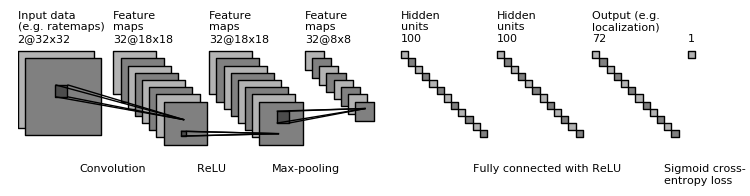
\includegraphics[scale=0.85]{images-data/convnet_fig}
\caption{Simple CNN architecture with one convolutional stage and two inner products}
\label{fig:introduction:convnet}
\end{figure}

\textbf{Convolutional stages.} We stack from one to three convolutional stages with their filter layers (hyperparameters: number of filters, size of filters, stride), non-linear layers (no hyperparameter for ReLUs) and dimension reduction layers using max pooling (hyperparameter: stride).

\textbf{Fully connected layers.} We stack from one to two inner products (hyperparameter: number of nodes) including dropout in the training phase.

\textbf{Activation layers.} They are sigmoid layers for the mixed sounds and softmax layers for the clean sounds. The softmax function allows to make a class stand out through the use of exponential coefficients,---thus achieving multiclass unilabel classification. The sigmoid function on the contrary only converts values from the last fully connected layer to related probabilities in the range $[0,1]$. In mathematical terms, we have for $j = 1,\dotsc,K$ (indices of the last inner product):
\begin{equation}
\left\{
\begin{aligned}
\text{Sigmoid: } & \sigma (\mathbf{z})_j = \frac{1}{1 + e^{-\mathbf{z}_j}} \\
\text{Softmax: } & \sigma (\mathbf{z})_j = \frac{e^{\mathbf{z}_j}}{\sum_{k=1}^K e^{\mathbf{z}_k}}
\label{eq:softmax}
\end{aligned}
\right.
\end{equation}

\subsection{Methods for hyperparameter optimization}
\label{methods:architecture:random}

\textbf{Manual optimization.} Going from coarse to fine on the hyperparameter ranges, we manually update the hyperparameters and check for the obtained accuracy. In addition to being relatively slow, this search is not optimal and only gives a sense of what may happen underneath. It requires an expert experience, as well as the knowledge of unwritten rules of thumbs.

\textbf{Grid search} consists of an exhaustive search on the whole hyperparameter space, each combination of hyperparameters being mapped to their respective accuracy. While this technique is particularly relevant for most machine learning algorithms, it is not well suited to neural networks where hyperparameters are numerous and lie in a highly dimensional space.

\textbf{Bayesian optimization} aims at efficiently navigating within the hyperparameter space. Spearmint \parencite{snoek2012practical} is an open-source Python library that can be used for that purpose. The Bayesian strategy treats the evaluation metrics as a random function with a prior over it (pre-knowledge). As models are trained, the prior is updated to form the posterior distribution which is in turn used to find the most appropriate hyperparameters that determine the next model to train.

\textbf{Random search} consists of a random search on the hyperparameter space. It is proved more efficient in time and computing power than a regular exhaustive grid search, because not all hyperparameters are equally important to tune \parencite{bergstra2012random}. We implemented a random search for Caffe and used it for models with clean and mixed sounds. For each architecture to investigate, the hyperparameters are randomly initialized, the network is trained for a given number of iterations and its performance is assessed through well-chosen evaluation metrics. When selecting models with random search, we proceed from coarse to fine in terms of depth and complexity of the tested architectures. In this manner, we can reuse the weights at each random iteration and need less learning iterations before convergence.